\section{How the obstructions scale with memory size}
\label{sec:memory}

Everything in Section~\ref{sec:source} concerns two sites. The construction
\eqref{eq:chem} is defined for every $N$, with $\binom{N+2}2$ states, and the
question is which of the two obstructions grows with $N$. This section answers
that for $2\le N\le8$ with exact rational certificates: the exposure floor is
almost flat in $N$, while the \emph{amplitude} required by the eraser grows by a
factor of nearly five. In particular the amplitude used in the two-site worked
example is certified insufficient, at any budget and any duration, at five to
eight sites.

\subsection{An exact test for the sign of the mean growth rate}

Let $A_e$ be the first-moment matrix \eqref{eq:meanmatrix} of the $N$-site
source at constant intrinsic erasure $e$, reconstructed from \eqref{eq:chem},
the binomial allocation law and the death rule. It is Metzler and, for $e>0$,
irreducible, because basal writing and intrinsic erasure connect every state to
every other. Then $M=-A_e$ is a $Z$-matrix, and the standard equivalence for
$Z$-matrices \citep[Ch.~6]{berman1994} gives
\begin{equation}\label{eq:mtest}
\begin{aligned}
 \spb(A_e)<0
 \ &\iff\ \text{$M$ is a nonsingular $M$-matrix}\\
 \ &\iff\ \text{all leading principal minors of $M$ are positive.}
\end{aligned}
\end{equation}
The right-hand condition is decided exactly by fraction-free elimination over
$\mathbb Q$, and the rates in \eqref{eq:chem} are rational whenever $e$ is.
Bisecting on $e$ with denominator $10^6$ therefore yields a rigorous bracket for
the critical erasure
\[
 e_c(N):=\inf\{e>0:\ \spb(A_e)<0\},
\]
which is well defined because $e\mapsto\spb(A_e)$ changes sign exactly once on
the tested range. The brackets are the first two numeric columns of
Table~\ref{tab:sites}; each was obtained by $21$ exact sign evaluations and each
is verified independently by a positive rational Collatz--Wielandt witness at
both endpoints, recorded in the data file \texttt{site\_certificates.json}.

\begin{table}[t]
\centering
\caption{Exact certificates for the $N$-site source \eqref{eq:chem}. The
critical erasure $e_c(N)$ is bracketed by the $M$-matrix test \eqref{eq:mtest}
at denominator $10^6$; $v_c=e_c-.01$ is the corresponding actuator amplitude.
The last two columns are a positive rational weight certificate
$A_{1/2}w\le-\gamma w$ at the common admissible erasure $e=1/2$, with
$C=w_{(N,0)}/w_{\min}$ as in Proposition~\ref{prop:weight}. All rows are exact
finite computations; $\gamma$ is exact at six decimals and $C$ is rounded up.}
\label{tab:sites}
\begin{tabular}{rrcccc}
\toprule
$N$ & states & $e_c(N)\in$ & $v_c(N)$ & $\gamma$ at $e=1/2$ & $C$ at $e=1/2$\\
\midrule
2 &  6 & $(.092750,.092751)$ & $.0827$ & $.166376$ & $3.7420$\\
3 & 10 & $(.188128,.188129)$ & $.1781$ & $.129493$ & $6.4630$\\
4 & 15 & $(.263685,.263686)$ & $.2537$ & $.095088$ & $9.3007$\\
5 & 21 & $(.324157,.324158)$ & $.3142$ & $.067868$ & $11.9061$\\
6 & 28 & $(.373695,.373696)$ & $.3637$ & $.046787$ & $14.2792$\\
7 & 36 & $(.415181,.415182)$ & $.4052$ & $.030242$ & $16.4792$\\
8 & 45 & $(.450572,.450573)$ & $.4406$ & $.017016$ & $18.5583$\\
\bottomrule
\end{tabular}
\end{table}

The two-site value reproduces, to the displayed resolution, the unique positive
root of the determinant polynomial
\begin{equation}\label{eq:detpoly}
 8{,}000{,}000{,}000\,e^5+7{,}688{,}000{,}000\,e^4+2{,}886{,}960{,}000\,e^3
 +439{,}939{,}800\,e^2-16{,}495{,}365\,e-5{,}182{,}134 ,
\end{equation}
which equals $5\cdot10^{9}\det A_e$ at $N=2$; its unique positive real root is
$.09275086931\ldots$, and the remaining four roots have negative real part.

\subsection{No policy eradicates below the threshold}

\begin{proposition}[Certified amplitude floors]\label{prop:ampfloor}
Consider the source \eqref{eq:chem} with baseline erasure $e=.01$ and eraser
amplitude $v_{\max}$, and let $\eta_{(N,0)}$ be the value in
Table~\ref{tab:amp}. For every predictable policy with values in $[0,v_{\max}]$,
including cell-specific policies, with no budget restriction and no horizon
restriction, survival from $n$ founders of the fully activating type $(N,0)$
satisfies
\[
 \Prob(\text{non-extinction})\ \ge\ 1-\bigl(1-\eta_{(N,0)}\bigr)^n ,
\]
and survival from a single founder of any type is at least
$1-\max_iq_i$. In particular, at the amplitude $v_{\max}=.29$ used in
Section~\ref{sec:twosite}, no policy whatsoever eradicates the $N$-site source
for $5\le N\le8$.
\end{proposition}

\begin{proof}
The explicit rational vectors $q$ in the data file \texttt{site\_certificates.json}
satisfy $\PhiB(q)\le0$ and $\Phi_{v_{\max}}(q)\le0$ with strictly negative
slacks in every coordinate, verified in exact arithmetic; the largest slack in
each case is reported in the data file. Theorem~\ref{thm:amp} and
Remark~\ref{rem:cellwise} then give the two displayed bounds.
\end{proof}

\begin{table}[t]
\centering
\caption{Certified amplitude floors: exact rational $q$ with
$\Phi_v(q)\le0$ for all $v\in[0,v_{\max}]$, so that no policy of that amplitude
eradicates at any budget or horizon. $\eta_{(N,0)}=1-q_{(N,0)}$ bounds survival
from one fully activating founder, and $1-\max_iq_i$ bounds it from the least
favourable founder type. The vectors were found by iterating the componentwise
maximum of the two fields to its minimal fixed point, retracted by the factor
$99/100$ along the segment of Lemma~\ref{lem:segment} and then verified exactly;
the retraction costs $1\%$ of $\eta$. The last row shows that the construction
remains feasible at $v_{\max}=.34$, close to the certified threshold
$v_c(6)=.363695\ldots$ of Table~\ref{tab:sites}.}
\label{tab:amp}
\begin{tabular}{rrrr}
\toprule
$N$ & $v_{\max}$ & $\eta_{(N,0)}$ & $1-\max_iq_i$\\
\midrule
2 & $.02$ & $.67850219$ & $.01263148$\\
2 & $.05$ & $.42726916$ & $.00771882$\\
2 & $.08$ & $.03785729$ & $.00067026$\\
\midrule
5 & $.29$ & $.17008641$ & $.00185216$\\
6 & $.29$ & $.45962721$ & $.00434343$\\
7 & $.29$ & $.61348974$ & $.00504729$\\
8 & $.29$ & $.70130311$ & $.00503641$\\
\midrule
6 & $.34$ & $.14866289$ & $.00133682$\\
\bottomrule
\end{tabular}
\end{table}

Two points deserve emphasis. First, the amplitude floors of
Table~\ref{tab:amp} are not statements about a particular constant action: they
hold against every predictable feedback policy, including ones that exploit the
non-monotonicity of \eqref{eq:taylor} by modulating the eraser, and they hold at
infinite budget. A mean-growth diagnostic at a single constant action --- for
instance the exact bracket $\spb(A_{.3})\in[239/10000,3/125]$ at $N=6$, or
$\spb(A_{.3})\in[-7/500,-139/10000]$ at $N=4$, both certified by positive
rational Collatz--Wielandt witnesses --- shows only that \emph{that} action
fails to contract, and leaves the policy question open. Theorem~\ref{thm:amp}
closes it.

Second, the failure at $5\le N\le8$ is a property of the source and not of a loose
certificate. The published four-site weight of the earlier two-site study
achieved $\gamma=.0132$ at $e=.3$, which is at least
$.0132/.014>94\%$ of the true mean decay rate at that action; almost none of the
deterioration between two and four sites is recoverable by searching harder for
a linear weight.

\begin{figure}[t]
\centering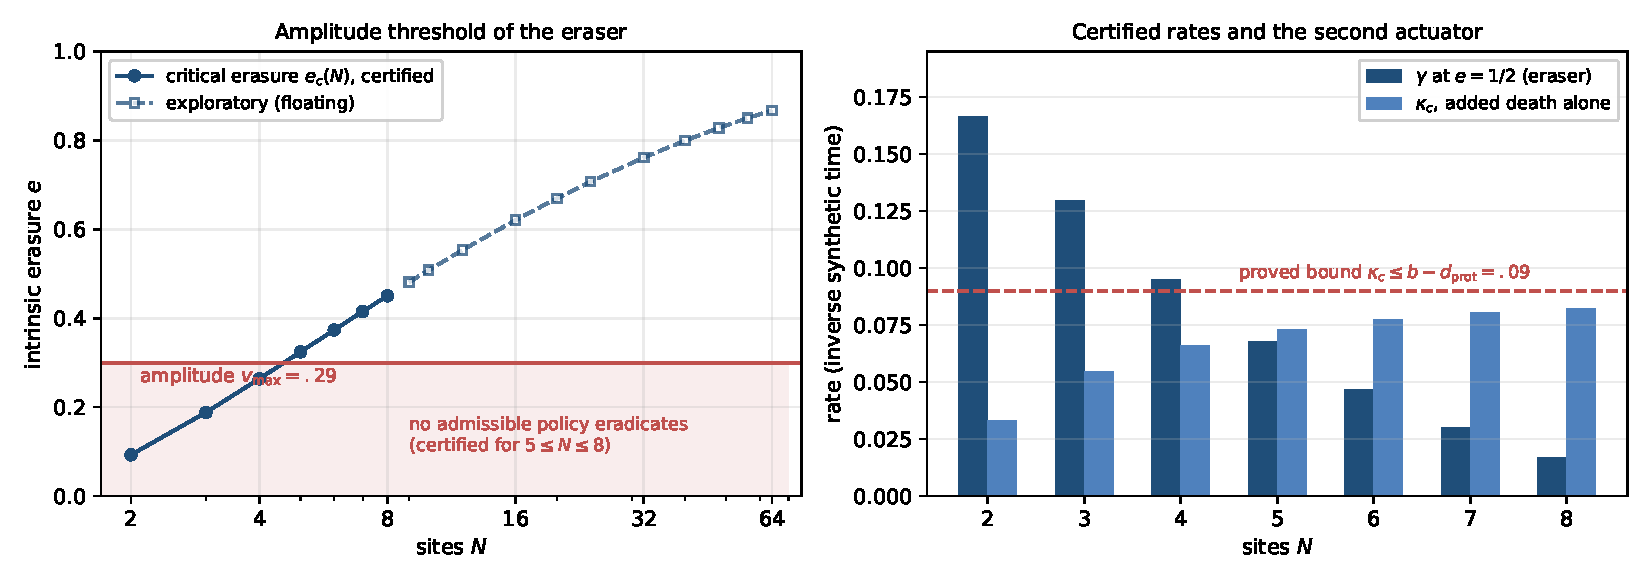
\includegraphics[width=\linewidth]{figures/sites.pdf}
\caption{Left: the eraser's critical intrinsic erasure against memory size.
Filled markers are the exact brackets of Table~\ref{tab:sites}; open markers are
exploratory floating eigenvalue computations for $9\le N\le64$ and are
diagnostics, not certificates. The shaded band is the amplitude used in the
two-site worked example; for $5\le N\le8$ the amplitude floors of
Table~\ref{tab:amp} certify that no policy in that band eradicates. Right:
certified mean contraction rate $\gamma$ of the eraser at the common erasure
$e=1/2$, and the certified threshold $\kappa_c$ of the added-death actuator
acting alone, which Proposition~\ref{prop:kappa} bounds by
$b-d_{\mathrm{prot}}=.09$ for every $N$.}
\label{fig:sites}
\end{figure}

\begin{remark}[Beyond the certified range]\label{rem:bigN}
Floating eigenvalue computations of $\spb(A_e)$, exact in the model but not
rounded rigorously, continue the first column of Table~\ref{tab:sites} as
$e_c\approx.508$ at $N=10$, $.621$ at $N=16$, $.762$ at $N=32$ and $.868$ at
$N=64$. The increments per unit of $\log N$ fall from about $.27$ to about
$.13$ over that range, so the sequence is increasing with decelerating
increments and we do not determine whether $e_c(N)$ remains bounded. What is
proved here is the monotone increase and the factor $4.86$ between $N=2$ and
$N=8$, together with the amplitude floors of Table~\ref{tab:amp}; no assertion
is made uniformly in $N$ for the eraser, and six or eight abstract sites are not
claimed to be a realistic chromatin domain.
\end{remark}

\subsection{The exposure floor barely moves}
\label{sec:expN}

Above the amplitude threshold the picture is different. Table~\ref{tab:expN}
gives, for each $N$, an exact baseline supersolution and the smallest admissible
$c$ for the eraser; the resulting necessary exposure at $n=1$, $\delta=.01$
increases by only $22\%$ between two and eight sites, against the factor $4.86$
in amplitude. Larger inherited state makes the actuator harder to \emph{power},
not appreciably more expensive to \emph{run}, in this source.

\begin{table}[t]
\centering
\caption{Exact baseline exposure certificates for the $N$-site source:
$\PhiB(q)\le0$ and $Rq\le c(1-q)$, with $\eta_{(N,0)}=1-q_{(N,0)}$ and
$B_{\mathrm{nec}}$ evaluated from \eqref{eq:necessary} at $n=1$, $\delta=.01$.
The $N=2$ row is the optimized certificate of Remark~\ref{rem:optcert}, which
supersedes \eqref{eq:q} by $0.54\%$. All vectors are in
the data file \texttt{site\_certificates.json}.}
\label{tab:expN}
\begin{tabular}{rrrr}
\toprule
$N$ & $\eta_{(N,0)}$ & $c$ & $B_{\mathrm{nec}}(1,.01)$\\
\midrule
2 & $.77849912$ & $.916533$ & $4.751365$\\
3 & $.85886565$ & $.884640$ & $5.033717$\\
4 & $.88009489$ & $.857113$ & $5.223867$\\
5 & $.88886370$ & $.832987$ & $5.387069$\\
6 & $.89308829$ & $.811604$ & $5.534843$\\
7 & $.89533756$ & $.792438$ & $5.671883$\\
8 & $.89661409$ & $.775121$ & $5.800437$\\
\bottomrule
\end{tabular}
\end{table}

The constructive side does deteriorate at a fixed amplitude: at the common
admissible erasure $e=1/2$, Table~\ref{tab:sites} gives $\gamma$ falling from
$.166$ to $.017$ and $C$ rising from $3.7$ to $18.6$, so
\eqref{eq:sufficient} yields $B_{\mathrm{suff}}(1,.01)$ growing from $17.4$ at
$N=2$ to $216.8$ at $N=8$. Raising the amplitude helps: a floating optimization
of $v_*/\gamma(v_*)$ over constant actions gives best free-horizon exposures of
about $17.1$ at $N=2$ (at $e=.43$), $27.8$ at $N=4$ (at $e=.74$) and $34.4$ at
$N=6$ (at $e=.91$). These are diagnostics; the certified rows are
Table~\ref{tab:sites}. Either way the eraser's sufficient exposure grows with
$N$ while its necessary exposure does not, so the constant gap widens and the
question of the true optimum becomes harder, not easier, with memory size.

\subsection{A second actuator removes the amplitude obstruction}
\label{sec:combo}

Corollary~\ref{cor:extensions} already admits several additive actuators. The
natural second one here adds death on the protected states,
\begin{equation}\label{eq:kappa}
 \Psi(x)=\kappa\odot(1-x),\qquad
 \kappa_i=\one_{\{a_i>r_i\}},
\end{equation}
with control $u\in[0,u_{\max}]$, so that the death rate in protected states
becomes $d_{\mathrm{prot}}+u$. This is a defined mathematical actuator, not a
claim that a known drug has that selectivity. Because $\kappa\le\one$ we may
take $c_\kappa=1$ in Corollary~\ref{cor:extensions}, so the necessary exposure
for this actuator is exactly $\log\bigl(\eta/(1-(1-\delta)^{1/n})\bigr)$ with
$\eta$ from Table~\ref{tab:expN}.

\begin{proposition}[Dimension-free sufficiency]\label{prop:kappa}
Let a finite-type source have binary division at rate $b$, death rates $d_i$,
count-preserving type changes, and an added-death actuator with nonnegative
indicator vector $\kappa$ as in \eqref{eq:kappa}, held at a constant value
$u=\kappa_*$. If
\[
 \gamma:=\min_i\bigl(d_i+\kappa_*\kappa_i-b\bigr)>0 ,
\]
then $\E|Z_t|\le|z|e^{-\gamma t}$, so $\Prob_z(|Z_t|>0)\le|z|e^{-\gamma t}$ and
extinction is almost sure. In the source \eqref{eq:chem}, where
$b=.1$, $d_{\mathrm{prot}}=.01$ and $d_{\mathrm{unprot}}=.3$, this holds for
every $N$ as soon as $\kappa_*>b-d_{\mathrm{prot}}=.09$, with
$\gamma=\min(\kappa_*-.09,\,.2)$ and $C=1$; hence
\begin{equation}\label{eq:kappasuff}
 B_{\mathrm{suff}}=\frac{\kappa_*}{\min(\kappa_*-.09,\ .2)}\,\log\frac n\delta ,
\end{equation}
minimized at $\kappa_*=.29$, where it equals $1.45\log(n/\delta)$ for every
number of sites.
\end{proposition}

\begin{proof}
Type changes preserve $|z|$ and binary division replaces one cell by two, so
$|Z_t|$ increases by one at rate $b|Z_t|$ and decreases by one at rate
$\sum_iZ_i(t)(d_i+\kappa_*\kappa_i)$. Hence
$\frac{d}{dt}\E|Z_t|=\E\sum_iZ_i(t)(b-d_i-\kappa_*\kappa_i)\le-\gamma\E|Z_t|$,
after the localization of Section~\ref{sec:model}, and Gronwall gives the
bound. Since $|Z_t|$ is integer valued, $\Prob(|Z_t|>0)\le\E|Z_t|$. This is
Proposition~\ref{prop:weight} with $w=\one$, so $C=1$; substituting
$t=\gamma^{-1}\log(n/\delta)$ and $B=\kappa_*t$ gives \eqref{eq:kappasuff}. In
\eqref{eq:chem} the protected states have $b-d=.09$ and the unprotected ones
$b-d=-.2$, giving the stated $\gamma$. Minimizing $\kappa_*/\min(\kappa_*-.09,.2)$
over $\kappa_*>.09$ gives the value $.29/.2=1.45$ at $\kappa_*=.29$.
\end{proof}

\begin{corollary}[Near-sharp exposure constant]\label{cor:sharpconst}
For the actuator \eqref{eq:kappa} in the source \eqref{eq:chem} with amplitude
$u_{\max}\ge.29$, at every $N\le8$,
\[
 \log\frac{\eta_{(N,0)}}{1-(1-\delta)^{1/n}}\ \le\ B^*(n,\delta)
 \ \le\ 1.45\,\log\frac n\delta ,
\]
so $\limsup_{n/\delta\to\infty}B^*(n,\delta)/\log(n/\delta)\le1.45$ while the
liminf is at least $1$. At $n=1$, $\delta=.01$ the certified bracket is
$4.354788\le B^*\le6.677497$, a ratio of $1.533$.
\end{corollary}

\begin{proof}
Combine Corollary~\ref{cor:extensions} with $c_\kappa=1$ and the values of
$\eta$ in Table~\ref{tab:expN} for the lower bound, and
Proposition~\ref{prop:kappa} for the upper. For the liminf use
\eqref{eq:rootbounds}, which gives
$B^*\ge\log(n/\delta)+\log(\eta/2)$.
\end{proof}

This is the sharpness statement that Proposition~\ref{prop:sharp} could not
supply inside a source with genuine inheritance: the exposure floor
\eqref{eq:main} is attained to within a factor $1.45$ by an explicit policy in
the molecular source, uniformly in the size of the inherited state, and the
leading order $\log(n/\delta)$ is exact.

Finally, a small amount of the second actuator repairs the eraser's failure
rather than replacing it. With the eraser held at $e=.3$ --- the amplitude that
Proposition~\ref{prop:ampfloor} certifies cannot eradicate on its own for
$5\le N\le8$ --- the added-death threshold is bracketed exactly at denominator
$10^6$ by
\[
 \kappa_c\in(.008894,.008895),\ (.024937,.024938),\ (.036344,.036345),\
 (.044765,.044766)
\]
for $N=5,6,7,8$ respectively. When the eraser is absent the corresponding
thresholds are
\[
 (.033181,\ .054493,\ .066139,\ .073090,\ .077472,\ .080374,\ .082373)
\]
for $N=2,\dots,8$ --- an increasing sequence that
Proposition~\ref{prop:kappa} caps at $.09$ for every $N$. At six sites an added
death of $.025$ on protected states therefore restores mean contraction where
an eraser amplitude of $.29$ provably cannot.
Additive certificate costs do not by themselves prove or disprove biological
synergy; synergy must be defined against a stated cost, dose pair, endpoint and
admissible policy class, and non-additive target interactions require their own
generator bounds.
